\ \\ [-5mm]
\begin{enumerate}
   \item Le thème étudié ici est le codage et la programmation, et plus particulièrement \og coder le déplacement d'un personnage sur un quadrillage \fg{}, dans le domaine \og espace et géométrie \fg.
   \item On peut par exemple choisir l'une des cartes \og programme \fg{}. Pour cette carte, on teste le programme sur le quadrillage 1, puis 2\dots {} jusqu'à trouver la bonne association. On poursuit de la même façon avec les autres cartes programme. On obtient : A - 2 \quad ; \quad B - 4 \quad ; \quad C - 3 \quad D - 1.
   \item Compétences requises :
   \begin{itemize}
      \item se repérer, décrire ou exécuter des déplacements, sur un
plan ou sur une carte ;
      \item connaître et utiliser le vocabulaire permettant de définir des
positions et des déplacements.
   \end{itemize}
   \item Exemples de difficultés :
   \begin{itemize}
      \item mauvaise compréhension de la consigne ;
      \item difficultés d'orientations (repérage relatif, dans un plan) ;
      \item choix de la procédure à utiliser pour arriver à ses fins.
   \end{itemize}
   \item On peut proposer à des élèves un quadrillage plus grand sur une feuille A4 avec un personnage de type Playmobil (donc orienté et pouvant se tenir debout) représentant Hercule ainsi qu'un jeton pour le pommier. L'élève devra tout d'abord placer le personnage et le jeton, puis tester les déplacements. L'avantage de ce matériel est un retour à une représentation en 3D, plus proche de la réalité et donc plus facilement transposable à la réalité. \\
   \hspace*{3cm} 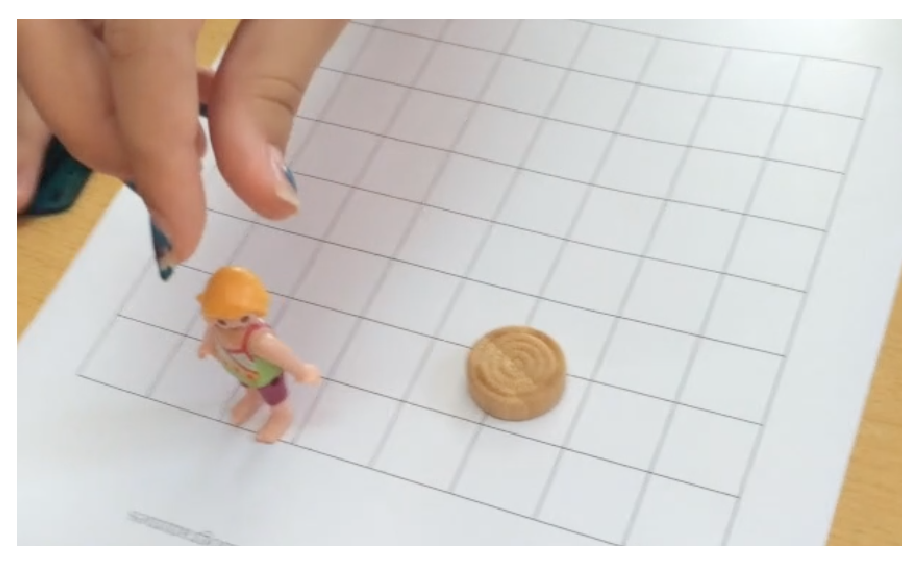
\includegraphics[width=11cm]{Geometrie_did/Images/Geo6_analyse_Playmobil} \\
   On peut également faire le même type d'action sur une nappe quadrillée sur laquelle les élèves peuvent se déplacer.
   \item On obtient les programmes minimum suivants : \\
   {\psset{unit=0.5}
   \hspace*{-0.5cm}
   \begin{pspicture}(0,2)(8,9.5)
      \rput(4,8.5){\bf A}
      \put(1,7){\dep}
      \put(1,6){\tg}
      \put(1,5){\av{1}}
      \put(1,4){\fin}
   \end{pspicture}
   \begin{pspicture}(0,2)(8,9.5)
      \rput(4,8.5){\bf B}
      \put(1,7){\dep}
      \put(1,6){\av{4}}
      \put(1,5){\fin}
   \end{pspicture}
   \begin{pspicture}(0,2)(8,9.5)
      \rput(4,8.5){\bf C}
      \put(1,7){\dep}
      \put(1,6){\av{4}}
      \put(1,5){\tg}
      \put(1,4){\av{2}}
      \put(1,3){\fin}
   \end{pspicture}
   \begin{pspicture}(0,2)(7,9.5)
      \rput(4,8.5){\bf D}
      \put(1,7){\dep}
      \put(1,3.5){\ret{2}}
      \put(2,5){\tg}
      \put(2,4){\av{2}}
      \put(1,2.5){\fin}
   \end{pspicture}}
\end{enumerate}
